\documentclass[reprint]{revtex4}
\usepackage{amsmath}
\usepackage{amssymb}
\usepackage{amsfonts}

%%%% GENERAL OPTIONS %%%%%%%%%%%%%%%%%%%
\usepackage[T1]{fontenc}
\usepackage{bm}
\usepackage{color}
\usepackage{graphicx}
\usepackage{hyperref}% add hypertext capabilities
\hypersetup{
    bookmarks=true,         % show bookmarks bar?
    unicode=false,          % non-Latin characters in Acrobat’s bookmarks
    pdftoolbar=true,        % show Acrobat’s toolbar?
    pdfmenubar=true,        % show Acrobat’s menu?
    pdffitwindow=false,     % window fit to page when opened
    pdfstartview={FitH},    % fits the width of the page to the window
    pdftitle={My title},    % title
    pdfauthor={Author},     % author
    pdfsubject={Subject},   % subject of the document
    pdfcreator={Creator},   % creator of the document
    pdfproducer={Producer}, % producer of the document
    pdfkeywords={keyword1} {key2} {key3}, % list of keywords
    pdfnewwindow=true,      % links in new PDF window
    colorlinks=true,        % false: boxed links; true: colored links
    linkcolor=black,      % color of internal links (change box color with linkbordercolor)
    citecolor=blue,         % color of links to bibliography
    filecolor=blue,      % color of file links
    urlcolor=blue           % color of external links
}
\usepackage{array}
\newcolumntype{C}[1]{>{\centering\arraybackslash$}p{#1}<{$}}

% some useful short commands
\newcommand{\unit}[1]{\boldsymbol{\widehat{\mathrm{#1}}}}
\newcommand{\todo}[1]{\textbf{\textcolor{red}{TODO: #1}}}
\newcommand{\fr}{\nu_{\textrm{r}}}
\newcommand{\fc}[1]{\nu_{#1}}
\newcommand{\tildefc}[1]{\tilde{\nu}_{#1}}
\newcommand{\E}{\hat{E}}
\newcommand{\frc}{\hat{\nu}_r}
\newcommand{\fcc}[1]{\hat{\nu}_{#1}}
\newcommand{\dif}{\bm{\partial}}
\newcommand{\ddif}{\bm{\partial^2}}
\newcommand{\e}{\mathbf{e}}
\newcommand{\red}[1]{\textbf{\textcolor{red}{#1}}}
\newcommand{\M}[2]{\mathbf{M}_{#1,#2}}%\mathsf
\newcommand{\bigzero}{\makebox(0,0){\text{\huge0}}}
\newcommand{\erf}{\textrm{erf}}

% For pointing out the revision changes
\newcommand{\eero}[1]{{\color{blue}#1}}
\newcommand{\diag}[1]{\mathbf{diag}\bm{\left[}#1\bm{\right]}}

\makeatother

\begin{document}

\title{Kinetic modeling of thermal quench}

%\author{E. Hirvijoki}
\date{\today}

\begin{abstract}
In these notes we take a simplified look at the kinetic processes that cause the plasma to cool down during thermal quench. We will assume two different mechanisms: (1) injection of cold particles, e.g., with pellets or neutral gas, (2) loss of particles due to plasma touching the wall. Simple models are used to simulate both these phenomena from the first principles, admitting efficient scans over wide parameter range. The simulations are then used to answer how many seed runaway electrons can be expected during thermal quench.
\end{abstract}

%\pacs{put Pacs here}

\maketitle
%\tableofcontents

\section{Model equations}
The electron distribution function is assumed to be afffected by electric field, Coulomb collisions, by a source term of cold electrons from ionization of neutrals, and by a sink term describing loss of particles to the wall mimicking loss of plasma confinement. For now, and for sake of simplicity, we will neglect the ion-electron collisions, as they are much more infrequent than the electon-electron collisions. The kinetic model is thus described by 
\begin{equation}
\frac{\partial f}{\partial t} -\frac{e\bm{E}}{m}\cdot\frac{\partial f}{\partial\bm{v}}= C[f,f]+s_{\textrm{cold}}-s_{\textrm{loss}},
\end{equation}
where the Fokker-Planck collision operator for like species collisions is given by 
\begin{equation}
C[f,f]=\left(\frac{e^4\ln\Lambda}{m^2\varepsilon_0^2}\right)\frac{\partial}{\partial\bm{v}}\cdot\left(\frac{\partial\phi}{\partial\bm{v}} f-\frac{\partial^2\psi}{\partial\bm{v}\partial\bm{v}}\cdot\frac{\partial f}{\partial\bm{v}}\right),
\end{equation}
and the Rosenbluth potentials are
\begin{equation}
\phi(\bm{v})=-\frac{1}{4\pi}\int f(\bm{v}')\frac{1}{\mid \bm{v}-\bm{v}'\mid}d\bm{v}',\qquad \psi(\bm{v})=-\frac{1}{8\pi}\int f(\bm{v}')\mid \bm{v}-\bm{v}'\mid d\bm{v}'.
\end{equation}
But before we proceed any further, it is good to start working with dimensionless quantities. 

We define $\bm{x}=\bm{v}/v_0$, where $v_0$ is a fixed reference velocity. Thus the volume element becomes $d\bm{v}=v_0^3d\bm{x}$ and any velocity space moment becomes $\int \bm{v}^n fd\bm{v}=v_0^{3+n}\int \bm{x}^nf d\bm{x}$. We also normalize the distribution function and define $F=v_0^3f/n_0$ so that any physical velocity space moment is given by $\int \bm{v}^n fd\bm{v}=n_0v_0^{n}\int \bm{x}^nF d\bm{x}$. If we also define normalized time $\tau=t/t_0$ where $t_0$ is a fixed reference time scale, we can write the dimensionless kinetic equation for $F$ according to 
\begin{equation}
\frac{\partial F}{\partial\tau}-\bar{\bm{E}}\cdot\nabla F\\=\nu C[F,F]+S
\end{equation}
where the normalized dimensionless quantities are
\begin{equation}
\bar{\bm{E}}=\frac{t_0e}{mv_0}\bm{E},\qquad \nu=\left(\frac{t_0n_0e^4\ln\Lambda}{v_0^3m^2\varepsilon_0^2}\right),\qquad S=\frac{v_0^3t_0}{n_0}s.
\end{equation}
The collision operator in the equation is then written simply
\begin{equation}
C[F,F]=\nabla\cdot\left(\nabla\Phi F-\nabla\nabla\Psi\cdot\nabla F\right)
\end{equation}
and the Rosenbluth potentials become
\begin{equation}
\Phi(\bm{x})=-\frac{1}{4\pi}\int F(\bm{y})\frac{1}{\mid \bm{x}-\bm{y}\mid}d\bm{y},\qquad \Psi(\bm{x})=-\frac{1}{8\pi}\int F(\bm{y})\mid \bm{x}-\bm{y}\mid d\bm{y},
\end{equation}
and satisfy the Poisson equations $\nabla^2\Phi = F$ and $\nabla^2\Psi =\Phi$.


\section{Weak formulation with backward Euler step}
Because the kinetic equation is stiff, the time discretization should be backward differentiation. We will use backward Euler, approximating the time derivative of distribution function at time instance $s$ with the expression $\partial F^{s}/\partial\tau\approx (F^{s}-F^{s-1})/\Delta \tau$. Further, because we cannot handle infinite domains, the space must be truncated. With that in mind, we multiply the kinetic equation with a test function $F^{\star}$ and integrate over the computational domain $\Omega$:
\begin{multline}
\int_{\Omega}F^{\star}\left(F^s -\Delta\tau S^s-\Delta\tau\bar{\bm{E}}\cdot\nabla F^s\right)d\bm{x}
+\nu\Delta\tau\int_{\Omega}\nabla F^{\star}\cdot\left(\nabla \Phi^s F^s-\nabla\nabla\Psi^s\cdot\nabla F^s\right)d\bm{x}\\
-\nu\Delta\tau\int_{\partial\Omega}F^{\star}\left(F^s\nabla\Phi^s-\nabla F^s\cdot\nabla\nabla\Psi^s\right)\cdot d\bm{\sigma}
=\int_{\Omega}F^{\star}F^{s-1}d\bm{x}.
\end{multline}
Similarly we do for the Poisson equations
\begin{align}
-\int_{\Omega}\nabla\Phi^s\cdot\nabla\Phi^{\star}d\bm{x}+\int_{\partial\Omega}\Phi^{\star}\nabla\Phi^s\cdot d\bm{\sigma}&=\int_{\Omega}F^s\Phi^{\star}d\bm{x}\\
-\int_{\Omega}\nabla\Psi^s\cdot\nabla\Psi^{\star}d\bm{x}+\int_{\partial\Omega}\Psi^{\star}\nabla\Psi^s\cdot d\bm{\sigma}&=\int_{\Omega}\Phi^s\Phi^{\star}d\bm{x}.
\end{align}
When we truncate the space, the distribution function $F$ is assumed to ``die off'' very fast and to be negligible outside the domain $\Omega$. This allows us to use the truncated definitions for the potential functions and to define Dirichlet conditions for the Poisson equations at the boundary $\partial\Omega$. 

To formulate the weak problems, we assume an $n$-th order Sobolev space for the test functions $V=\{v\in H^n(\Omega) \mid v(\partial\Omega)=0 \}$ which, together with the conditions that $\Phi$ and $\Psi$ are smooth functions, allows us to get rid of the boundary terms in the Poisson equations: A Dirichlet condition is needed to make the potentials unique, the Neumann condition is not needed. The Weak formulation for the first Rosenbluth potential is then 
\begin{align}
&-\int_{\Omega}\nabla\Phi^s\cdot\nabla\Phi^{\star}d\bm{x}=\int_{\Omega}F^s\Phi^{\star}d\bm{x}, \quad \bm{x}\in\Omega, \quad \forall \Phi^{\star}\in V\\
&\Phi^s(\bm{x})=-\frac{1}{4\pi}\int \frac{F^s(\bm{y})}{\mid \bm{x}-\bm{y}\mid}d\bm{y}, \quad \bm{x}\in\partial\Omega,
\end{align}
and for the second potential we have similarly
\begin{align}
&-\int_{\Omega}\nabla\Psi^s\cdot\nabla\Psi^{\star}d\bm{x}=\int_{\Omega}\Phi^s\Psi^{\star}d\bm{x}, \quad \bm{x}\in\Omega, \quad \forall \Psi^{\star}\in V\\
&\Psi^s(\bm{x})=-\frac{1}{8\pi}\int F^s(\bm{y})\mid \bm{x}-\bm{y}\mid d\bm{y}, \quad \bm{x}\in\partial\Omega.
\end{align}
Assuming the distribution function to vanish at the boundary, i.e., $F^s(\partial\Omega)=0$, the equation for $F^s$ becomes
\begin{multline}
\int_{\Omega}F^{\star}\left(F^s -\Delta\tau S^s-\Delta\tau\bar{\bm{E}}\cdot\nabla F^s\right)d\bm{x}
+\nu\Delta\tau\int_{\Omega}\nabla F^{\star}\cdot\left(\nabla \Phi^s F^s-\nabla\nabla\Psi^s\cdot\nabla F^s\right)d\bm{x}\\
=\int_{\Omega}F^{\star}F^{s-1}d\bm{x}, \quad \bm{x}\in\Omega, \quad \forall F^{\star}\in V.
\end{multline}

For a general set of curvilinear coordinates $x^{i}(x^1,x^2,x^3)$ with a metric tensor $g_{ij}$, the collision operator can be conveniently expressed as 
\begin{equation}
C=\sqrt{g}^{-1}\partial_i\left[\sqrt{g}K^if-\sqrt{g}D^{ij}\partial_jf\right],
\end{equation}
where the covariant components of the friction and diffusion terms are
\begin{equation}
K^i=\e^{i}\cdot \nabla\Phi = g^{ij}\partial_j\Phi,\qquad D^{ij}=\e^i\cdot\nabla\nabla\Psi\cdot\e^j=g^{ik}g^{j\ell}\left(\partial^2_{k\ell}\Psi-\Gamma^m_{k\ell}\partial_m \Psi\right).
\end{equation}
and $\Gamma^i_{jk}=\partial_k \e_j\cdot\e^i=g^{i\ell}\left(\partial_k g_{\ell j}+\partial_j g_{\ell k}-\partial_{\ell} g_{jk}\right)/2$ is the Christoffel symbol of the second kind.

In our case, the distribution function will have symmetry along the axis of the electric field, and natural choice of coordinates being either spherical or cylindrical. It is thus usefull to express the weak forms directly in curvilinear coordinates and we get:
\begin{itemize}
\item[1.] Weak formulation for the distribution function: 
$F^s(\partial\Omega)=0$.
\begin{multline}
\int_{\Omega}F^{\star}\left(F^s -\Delta\tau S^s-\Delta\tau\bar{E}^i\partial_i F^s\right)\sqrt{g}dx^1dx^2dx^3\\
+\nu\Delta\tau\int_{\Omega}\partial_iF^{\star}\left[g^{ij}\partial_j\Phi^s F^s-g^{ik}g^{j\ell}\left(\partial^2_{k\ell}\Psi^s-\Gamma^m_{k\ell}\partial_m \Psi^s\right)\partial_j F^s\right]\sqrt{g}dx^1dx^2dx^3\\
=\int_{\Omega}F^{\star}F^{s-1}\sqrt{g}dx^1dx^2dx^3, \quad \bm{x}\in\Omega, \quad \forall F^{\star}\in V,
\end{multline}
\item[2.] Weak formulation for the first Rosenbluth potential:
\begin{align}
-\int_{\Omega}\partial_i\Phi^sg^{ij}\partial_j\Phi^{\star}\sqrt{g}dx^1dx^2dx^3&=\int_{\Omega}F^s\Phi^{\star}\sqrt{g}dx^1dx^2dx^3, \quad \bm{x}\in\Omega, \quad \forall \Phi^{\star}\in V\\
\Phi^s(\bm{x})&=-\frac{1}{4\pi}\int \frac{F^s(\bm{y})}{\mid \bm{x}-\bm{y}\mid}\sqrt{g}dy^1dy^2dy^3, \quad \bm{x}\in\partial\Omega,
\end{align}
\item[3.] Weak formulation for the second Rosenbluth potential:
\begin{align}
-\int_{\Omega}\partial_i\Psi^s g^{ij}\partial_j\Psi^{\star}\sqrt{g}dx^1dx^2dx^3&=\int_{\Omega}\Phi^s\Psi^{\star}\sqrt{g}dx^1dx^2dx^3, \quad \bm{x}\in\Omega, \quad \forall \Psi^{\star}\in V\\
\Psi^s(\bm{x})&=-\frac{1}{8\pi}\int F^s(\bm{y})\mid \bm{x}-\bm{y}\mid \sqrt{g}dy^1dy^2dy^3, \quad \bm{x}\in\partial\Omega.
\end{align}
\end{itemize}

The only complication in our system is the nonlinearity: because the potential functions depend on $F^s$, the weak formulation for $F^s$ is not linear. Fortunately, there is a simple recipe for solving these kind of problems, namely the Banach or Picard-Lindel\"of iteration. One starts with some function $\tilde{F}$, uses that to compute approximations for the potential functions, and solves the weak problem for $F^s$ with simple matrix inversion. Then this solution is used to compute new values for the potentials, and an iterative method is ready. For our particular case this is expected to work reasonably well because the distribution is not expected to change radically due to collisions from one time point to the next. And since we have an initial state for the distribution function, our guess for the potentials is typically close to the correct expression. It is not uncommon at all to actually use only the first iteration, in which case the backward time differentiation results in an equation which can be solved with one matrix solve. Nevertheless, more sophisticated approaches also exist.

\section{Spherically symmetric cooling down}
The most simple model for the cooling-down process is to assume a zero electric field and a spherically symmetric source of cold particles which drives equilibration of the temperature. The whole kinetic equation will be spherically symmetric, and the weak formulations become quite compact. 

In short, we truncate the domain to be a ball limited at radius $\mid\bm{x}\mid = c$ which then gives
\begin{itemize}
\item[1.] the weak formulation for the distribution function: $F^s(c)=0$
\begin{multline}
\int_0^cF^{\star}(F^s-\Delta\tau S^s)r^2dr+\nu\Delta\tau\int_0^c\partial_rF^{\star}\partial_r\Phi^s F^sr^2dr-\nu\Delta\tau\int_0^cr^2\partial_rF^{\star}\partial^2_{rr}\Psi^k\partial_rF^kdv
\\=\int_0^cr^2F^{\star}F^{k-1}dr, \quad \forall F^{\star}\in V
\end{multline}
\item[2.] the weak formulation for the first Rosenbluht potential:
\begin{align}
-\int_0^c\partial_r\Phi^s\partial_r\Phi^{\star}r^2dr&=\int_0^c\Phi^{\star}F^s, \quad \forall \Phi^{\star}\in V\\
\Phi^s(c)&=-\frac{1}{c}\int_0^c F^sr^2 dr.
\end{align}
\item[3.] the weak formulation for the second Rosenbluth potential:
\begin{align}
-\int_0^c\partial_r\Psi^s\partial_r\Psi^{\star}r^2dr&=\int_0^c\Psi^{\star}\Phi^s, \quad \forall \Psi^{\star}\in V\\
\Psi^s(c)&=-\frac{c}{2}\int_0^c  F^s r^2dr-\frac{1}{6c}\int_0^c r^2 F^s r^2dr.
\end{align}
\end{itemize}
Here we have to keep in mind that the Green's function solutions for the Rosenbluth potentials are truncated to be consistent with the assumption that $F$ vanishes outside the domain 
% Assuming that the distribution function is independent of the gyroangle $\theta$, the friction terms in $(r,\xi)$ coordinates are given by
% \begin{align}
% K^r&=\partial_r\Phi\\
% K^{\xi}&=\frac{1-\xi^2}{r^2}\partial_{\xi}\Phi
% \end{align}
% and the diffusion tensor has the components
% \begin{align}
% D^{rr}&=\partial^2_{rr}\Psi\\
% D^{r\xi}&=D^{\xi r}=\frac{1-\xi^2}{r^2}\left(\partial^2_{r\xi}\Psi-\frac{1}{r}\partial_{\xi}\Psi\right)\\
% D^{\xi\xi}&=\left(\frac{1-\xi^2}{r^2}\right)^2\left(\partial^2_{\xi\xi}\Psi-\frac{\xi}{1-\xi^2}\partial_{\xi}\Psi+\frac{r}{1-\xi^2}\partial_r\Psi\right)
% \end{align}

% \subsection{Spherically symmetric case}
% If the initial distribution function has spherical symmetry, and there is nothing to drive non-isotropy, we can make a significant simplification to the equations: the friction has only one component 
% \begin{equation}
% K^r=\partial_r\Phi
% \end{equation}
% and we only need one component for the diffusion tensor
% \begin{equation}
% D^{rr}=\partial^2_{rr}\Psi.
% \end{equation}
% Thus the nonlinear collision operator can be expressed as
% \begin{equation}
% C[f,f]=r^{-2}\partial_r\left(r^2\partial_r\Phi\ F-r^2\partial^2_{rr}\Psi\ \partial_r F\right),
% \end{equation}
% and the potentials satisfy the differential equations
% \begin{align}
% r^{-2}\partial_r\left(r^2\partial_r\Phi\right)&=F\\
% r^{-2}\partial_r\left(r^2\partial_r\Psi\right)&=\Phi
% \end{align}
% The potential $\Phi$ has a simple Green's function solution
% \begin{equation}
% \Phi(r)=-\frac{1}{r}\int_0^r y^2 F(y) dy-\int_r^\infty y F(y) dy
% \end{equation}
% and for the potential $\Psi$ one finds 
% \begin{multline}
% \Psi(r)=-\frac{r}{2}\int_0^r y^2 F(y) dy-\frac{1}{6r}\int_0^r y^4 F(y) dy-\frac{1}{2}\int_r^\infty y^3 F(y) dy
% -\frac{r^2}{6}\int_r^\infty y F(y) dy.
% \end{multline}
% Assuming that the distribution function dies off quickly enough (exponentially), the Green's function solutions can be used to determine boundary conditions for the Poisson equations.

% \section{Weak formulation for the spherically symmetric potential functions}
% We first take a look at the spherically symmetric Poisson equation. The first approximation we have to do is the truncation of the originally infinite speed domain $[0,\infty )$ to a finite one $[0,c]$. Assuming that the distribution function $f$ dies off exponentially this approximation can be tolerated as long as $c$ is chosen to be ``large enough''. We then redefine the strong form for the Poisson equations
% \begin{align}
% r^{-2}\partial_r\left(r^2\partial_r\Phi\right)&=F, \quad r \in [0,c]\\
% \partial_r\Phi&=0, \quad r=0\\
% \Phi&=\Phi_c, \quad r=c ,
% \end{align}
% where the Neumann condition at $r=0$ rises because $\Phi$ should be continuous and smooth, and the Dirichlet condition at $r=c$ can be computed from the infinite space Green's function solution
% \begin{equation}
% \Phi(c)=-\frac{1}{c}\int_0^c y^2 F(y) dy.
% \end{equation}
% This form assumes that the distribution function is vanishingly small outside the region $[0,c]$ allowing truncation of the Green's function solution. Another approach would be to use Neuman condition also at the boundary $r=c$, since the Green's function solution would also provide
% \begin{equation}
% \partial_r\Phi(c)=\frac{1}{c^2}\int_0^c y^2 F(y) dy.
% \end{equation}
% This approach, however, might not be the best one, since it would not provide a unique solution to the Poisson problem, and unique solution is useful if $\Phi$ is to be used as the source function in the Poisson problem for $\Psi$.

% \subsection{The potential equations}
% With the strong form of the Poisson problem defined, we can start constructing the weak formulation. Multiplying the Poisson problem with a test function $\Phi^{\star}$, integrating over the domain $r\in[0,c]$, and using partial integration, we arrive at
% \begin{equation}
% -\int_o^c r^2\partial_r\Phi\partial_r\Phi^{\star} dr+\left[r^2\Phi^{\star}\partial_r\Phi\right]_0^c=\int_0^cr^2f\Phi^{\star} dr.
% \end{equation}
% Immediately, we see how the factor $r^2$ in the ``boundary term'' reflects the fact that we are considering an originally 3-D problem with symmetry: the $r^2$ factor makes sure that the boundary condition we reasoned at $r=0$ is built in and that the boundary term at $r=0$ never contributes to the weak form, as if we used the information. 

% The weak form does not allow us to directly include the Diriclet condition at $r=c$, and since we don't ``know'' the value $\partial_r\Phi(c)$ it has to be excluded from the weak form. Thus we have to choose our test function $\Phi^{\star}$ so that it belongs to a vector space $V=\{v(r)\in H^n([0,c])\mid v(c)=0 \}$ with $n$ at least one. In plain english: the test function has to satisfy $\Phi^{\star}(c)=0$ and has to belong into Sobolev space of order at least $1$, meaning that the function and its first derivative are $L^2$ integrable with respect to some measure, which in our case is $r^2dr$. Since we cannot embed the Diriclet condition into the weak formulation, it has to be included explicitly. All this means is that our final form for the weak problem is: find $\Phi$, so that 
% \begin{align}
% &A(\partial_r\Phi,\partial_r\Phi^{\star})=L_F(\Phi^{\star}), \quad \forall \Phi^{\star}\in V\\
% &\Phi(c)=-\frac{1}{c}\int_0^c r^2 F(r) dr.
% \end{align}
% where the bilinear form $A(\Xi,\Pi)$ and the measure $L(\Xi)$ are defined according to
% \begin{align}
% A(\Xi,\Pi)&=-\int_0^c \Xi \Pi r^2 dr\\
% L_F(\Xi)&=\int_0^c F \Xi r^2 dr
% \end{align}

\begin{figure}[!h]
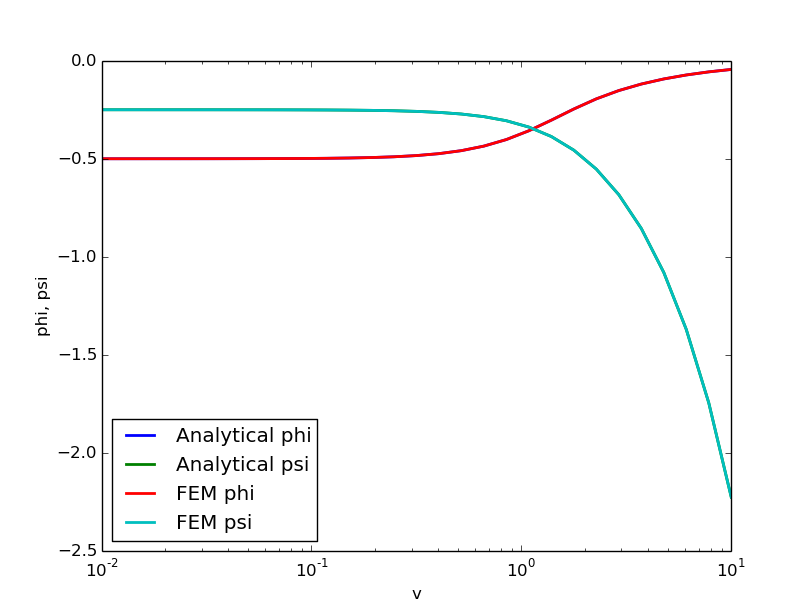
\includegraphics[width=0.45\textwidth]{fig/phi_psi.png}
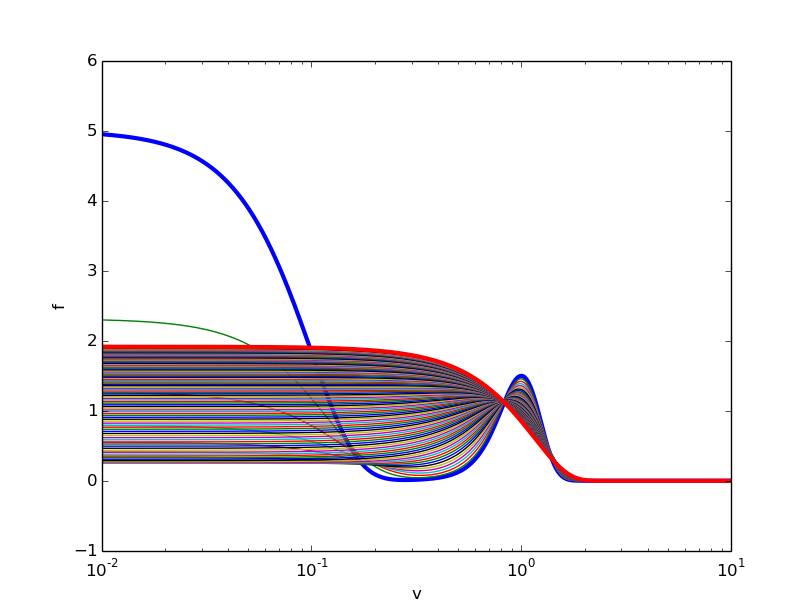
\includegraphics[width=0.45\textwidth]{fig/f_relaxation.png}
\caption{(left) Comparison of analytical (blue, green) and FEM (red, cyan) solution of the Rosenbluth potentials $\Phi$ and $\Psi$ in a Maxwellian plasma. For both potentials the FEM solutions completely overlap with the analytical expressions, and the solutions are numerically stable also at the point $r=0$. (right) Relaxation of a spherically symmetric non-Maxwellian initial state (thick blue) towards equilibrium (thick red).}
\label{fig:spherical_test}
\end{figure}
The first thing to do is to test the truncated Poisson equations given an analytical distribution function. The most relevant case is to take $F=\exp(-r^2)$, so that the analytical solutions computed from the exact infinite space Greens functions are
\begin{equation}
\Phi=-\frac{\sqrt{\pi}\erf(r)}{4r},\qquad
\Psi=-\frac{2r\exp(-r^2)+\sqrt{\pi}(1+2r^2)\erf(r)}{16r}
\end{equation}
Using the finite element library \rm{FEniCS}~\cite{dolfin_ref} we solve the truncated potential functions using the weak formulation and compare the result to the analytical solution in Fig.~\ref{fig:spherical_test}. The numerical truncated solution appears to be good, achieving six correct digits at $r=0$ with second order elements and 30 logarithmically placed mesh points. As a second test, we check the relaxation of nonlinear initial state to equilbrium. Setting $F_0(r)=1.5\exp\left[-10(r-1)^2\right]+5\exp\left[-100r^2\right]$, Fig.~\ref{fig:spherical_test} shows that the backward time differentiation is very robust and would allow very long time steps, as the few first steps demonstrate. Also the density is conserved to machine precision.

Next we add a source term for cold electrons. Using a simple gaussian source with a narrow width and constant rate, we observe the temperature to drop as expected when the total density is increased (see Fig.~\ref{fig:spherical_cooling_test}). At the same time the distribution function starts to develop a tail because the collisionality is different for the high-energy particles.
\begin{figure}[!h]
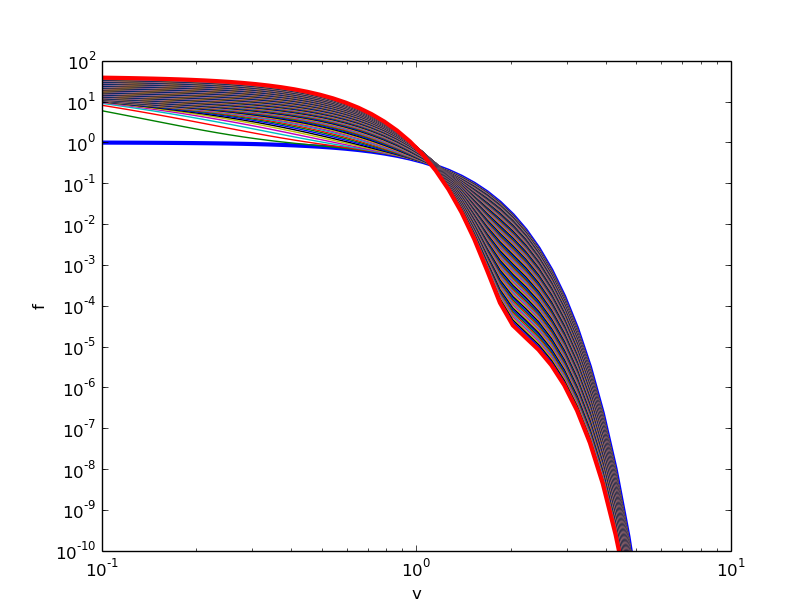
\includegraphics[width=0.45\textwidth]{fig/f_cooling_down.png}
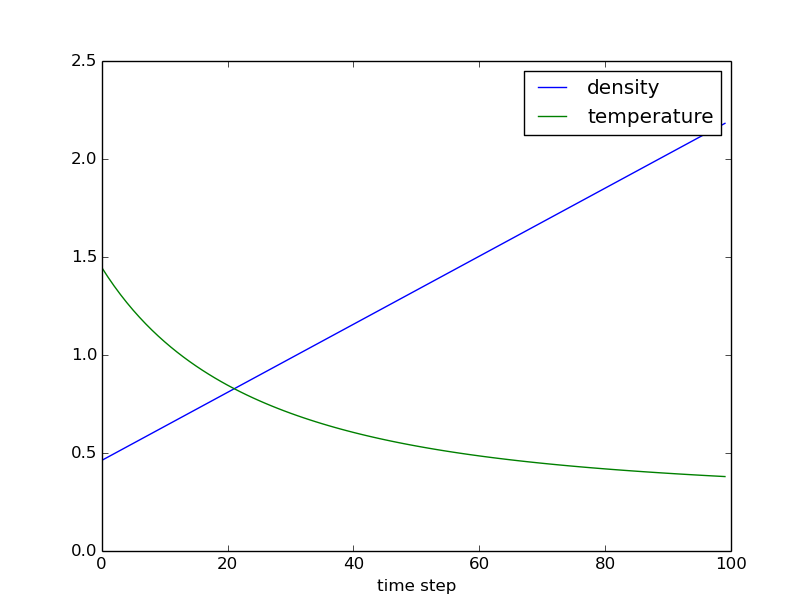
\includegraphics[width=0.45\textwidth]{fig/spherically_symmetric_temperature_relaxation.png}
\caption{(Left) Time evolution of the spherically symmetric distribution function due to spherically symmetric source of cold particles. The cold population is increased at constant rate. Thick blue is the initial state and thick red the final time instance. (Right) Temperature and density evolution during the cooling-down.}
\label{fig:spherical_cooling_test}
\end{figure}


\section{Cylindrical velocity space}
Because the electric field in the runaway problem points to the direction parallel to the magnetic field, the cylindrical coordinate with the z-axis directed along the electric field is a natural choice. 

In cylindrically symmetric case, assuming the electric field to be parallel to the $z$-axis, we find
\begin{itemize}
\item[1.] weak formulation for the distribution function: $F^s(\partial\Omega)=0$.
\begin{multline}
\iint_{\Omega}F^{\star}\left(F^s -\Delta\tau S^s-\Delta\tau\bar{E}^z\partial_z F^s\right)\rho d\rho dz
+\nu\Delta\tau\iint_{\Omega}\left(\partial_{\rho}F^{\star}\partial_{\rho}\Phi^s+\partial_{z}F^{\star}\partial_{z}\Phi^s\right) F^s\rho d\rho dz\\
-\nu\Delta\tau\iint_{\Omega}\left[\partial_{\rho}F^{\star}\partial^2_{\rho\rho}\Psi^s\partial_{\rho} F^s+\partial^2_{\rho z}\Psi^s\left(\partial_{\rho}F^{\star}\partial_{z} F^s+\partial_{z}F^{\star}\partial_{\rho} F^s\right)+\partial_{z}F^{\star}\partial^2_{zz}\Psi^s\partial_{z} F^s\right] \rho d\rho dz\\
=\iint_{\Omega}F^{\star}F^{s-1}\rho d\rho dz, \quad (\rho,z)\in\Omega, \quad \forall F^{\star}\in V,
\end{multline}
\item[2.] Weak formulation for the first Rosenbluth potential:
\begin{align}
-\iint_{\Omega} \left(\partial_z\Phi\partial_z\Phi^{\star}+\partial_{\rho}\Phi\partial_{\rho}\Phi^{\star}\right)\rho d\rho dz&=\iint F\Phi^{\star} \rho d\rho dz, \quad (\rho,z)\in\Omega, \quad \forall \Phi^{\star}\in V\\
 \Phi(\rho,z)&=-\frac{1}{\pi}\iint_{\Omega} F(\rho',z')\frac{K(k)}{\sqrt{(z-z')^2+(\rho+\rho')^2}}\rho'd\rho'dz', \quad (\rho,z)\in\partial\Omega,
\end{align}
\item[3.] Weak formulation for the second Rosenbluth potential:
\begin{align}
-\iint_{\Omega} \left(\partial_z\Psi\partial_z\Psi^{\star}+\partial_{\rho}\Psi\partial_{\rho}\Psi^{\star}\right)\rho d\rho dz&=\iint_{\Omega} \Phi\Psi^{\star} \rho d\rho dz, \quad (\rho,z)\in\Omega, \quad \forall \Phi^{\star}\in V\\
 \Phi(\rho,z)&=-\frac{1}{2\pi}\iint_{\Omega} F(\rho',z')E(k)\sqrt{(z-z')^2+(\rho+\rho')^2}\rho'd\rho'dz', \quad (\rho,z)\in\partial\Omega,
\end{align}
\end{itemize}
where $k=(4\rho\rho')/[(z-z')^2+(\rho+\rho')^2]$ and $K(k)$ and $E(k)$ are the complete elliptic integrals of the first and second kind as defined in Mathematica.

\newpage
\appendix




\section{Cylindrical coordinates}
The cylindrical coordinates $x^i=(\rho,\theta,z)$ relate back to Cartesian coordinates according to
\begin{equation}
x=\rho\sin\theta, \quad y=\rho\sin\theta
\end{equation}
so that the metric tensor has non-zero components
\begin{equation}
g_{\rho\rho}=1,\quad g_{\theta\theta}=\rho^2,\quad g_{zz}=1,
\end{equation}
and the nonzero Christoffel symbols are
\begin{align}
\Gamma^{\rho}_{\theta\theta}&=-\rho\\
\Gamma^{\theta}_{\rho\theta}&=\Gamma^{\theta}_{\theta\rho}=1/\rho.
\end{align}
The distance between two points is given by
\begin{equation}
\mid \bm{x}-\bm{x}'\mid=\sqrt{(z-z')^2+(\rho+\rho')^2}\sqrt{1-k\cos^2[(\theta-\theta')/2]},
\end{equation}
where
\begin{equation}
k=\frac{4\rho\rho'}{(z-z')^2+(\rho+\rho')^2}
\end{equation}
The angular integrals are thus
\begin{align}
\int_0^{2\pi}\mid \bm{x}-\bm{x}'\mid d\theta'&=4E(k)\sqrt{(z-z')^2+(\rho+\rho')^2},\\
\int_0^{2\pi}\mid \bm{x}-\bm{x}'\mid^{-1} d\theta'&=\frac{4K(k)}{\sqrt{(z-z')^2+(\rho+\rho')^2}},
\end{align}
where $K(k)$ and $E(k)$ are the complete elliptic integrals of the first and second kind as defined in Mathematica.

\section{Spherical coordinates}
 The spherical coordinates $x^i=(x,\xi,\theta)$ relate back to Cartesian coordinates according to 
\begin{equation}
 x=r\sqrt{1-\xi^2}\cos\theta,\quad y=r\sqrt{1-\xi^2}\sin\theta,\quad z=\xi r,
\end{equation}
and the metric is given by
\begin{equation}
g_{rr}=1,\quad g_{\xi\xi}=\frac{r^2}{1-\xi^2},\quad g_{\theta\theta}=r^2\left(1-\xi^2\right).
\end{equation}
The nonzero Christoffel symbols are
\begin{align}
\Gamma^r_{\xi\xi}&=-r/(1-\xi^2)\\
\Gamma^r_{\xi\theta}&=-r\sqrt{1-\xi^2}\\
\Gamma^{\xi}_{r\xi}&=\Gamma^{\xi}_{\xi r}=1/r\\
\Gamma^{\xi}_{\xi\xi}&=\xi/(1-\xi^2)\\
\Gamma^{\xi}_{\theta\theta}&=\xi\sqrt{1-\xi^2}\\
\Gamma^{\theta}_{r\theta}&=\Gamma^{\theta}_{\theta r}=1/r\\
\Gamma^{\theta}_{\xi\theta}&=\Gamma^{\theta}_{\theta \xi}=-\xi/(1-\xi^2)
\end{align}

\bibliographystyle{unsrt}
\bibliography{bibfile}

\end{document}
